50. $\cfrac{1}{(4-x^2)(x-2)}\leqslant\cfrac{1}{2-x} \Leftrightarrow\cfrac{-1}{(x-2)^2(x+2)}-\cfrac{1}{2-x}\leqslant0\Leftrightarrow
\cfrac{-1+x^2-4}{(x-2)^2(x+2)}\leqslant0\Leftrightarrow$\\$\cfrac{(x-\sqrt{5})(x+\sqrt{5})}{(x-2)^2(x+2)}\leqslant0.$\\ Применив метод интервалов, найдём ответ:
\begin{figure}[ht!]
\center{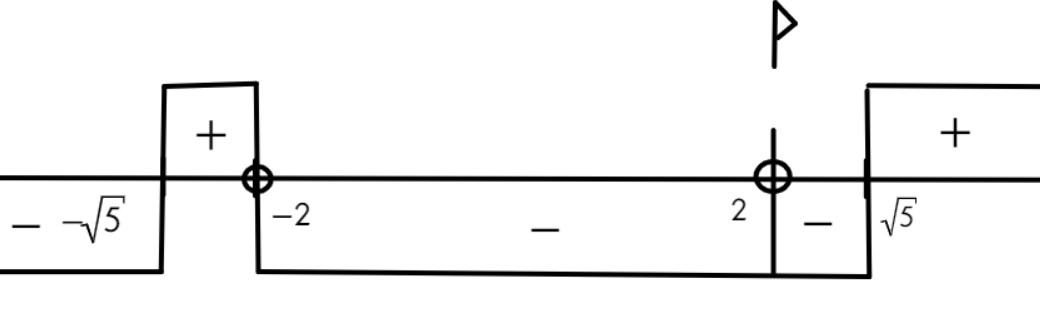
\includegraphics[scale=0.35]{int50.png}}
\end{figure}
$x\in(-\infty;-\sqrt{5}]\cup(-2;2)\cup(2;\sqrt{5}].$\\
